%!TEX root = ../../diachron-D5_2.tex

\subsection{Sequential Stream Processor}
\label{sec:StreamProcessor} 
In order to accurately assess linked dataset for quality measures, the assessment should on all triples in the assessed datasets.
One must keep in mind that the computation of metrics on large datasets might be computationally expensive; thus, such stream processors computing dataset's quality must be scalable.
In Figure~\ref{fig:closerLook}, a closer look towards the quality assessment process is illustrated.
A user first chooses a dataset and the metrics which are required for the assessment of quality.
The submitted information is passed to the Quality Framework via its API and initialise the processing unit (stream processor) in the core framework.
The stream processor is then initialised by: (1) creating the necessary objects in memory, and (2) initialise the chosen metrics. 
In Figure~\ref{fig:closerLook}, ``Metric 1'' is shadowed out – to illustrate that it was not chosen by the user for this particular use case.
Once the objects created, the stream processor fetches the dataset and in a sequential fashion it starts streaming quads one by one to all initialised metrics in parallel.
After all statements are assessed, the semantic annotation unit requests the metric value for each metric and creates (or updates – in case the dataset already has one) the Quality Graph.
This named graph represents the quality metadata of a dataset using the representation defined in Section~\ref{sec:DAQ}, and it is stored in the dataset itself.
Having this metadata, it will allow us to rank and crawl datasets based on different quality attributes.

\begin{figure*}[tbph]
\center
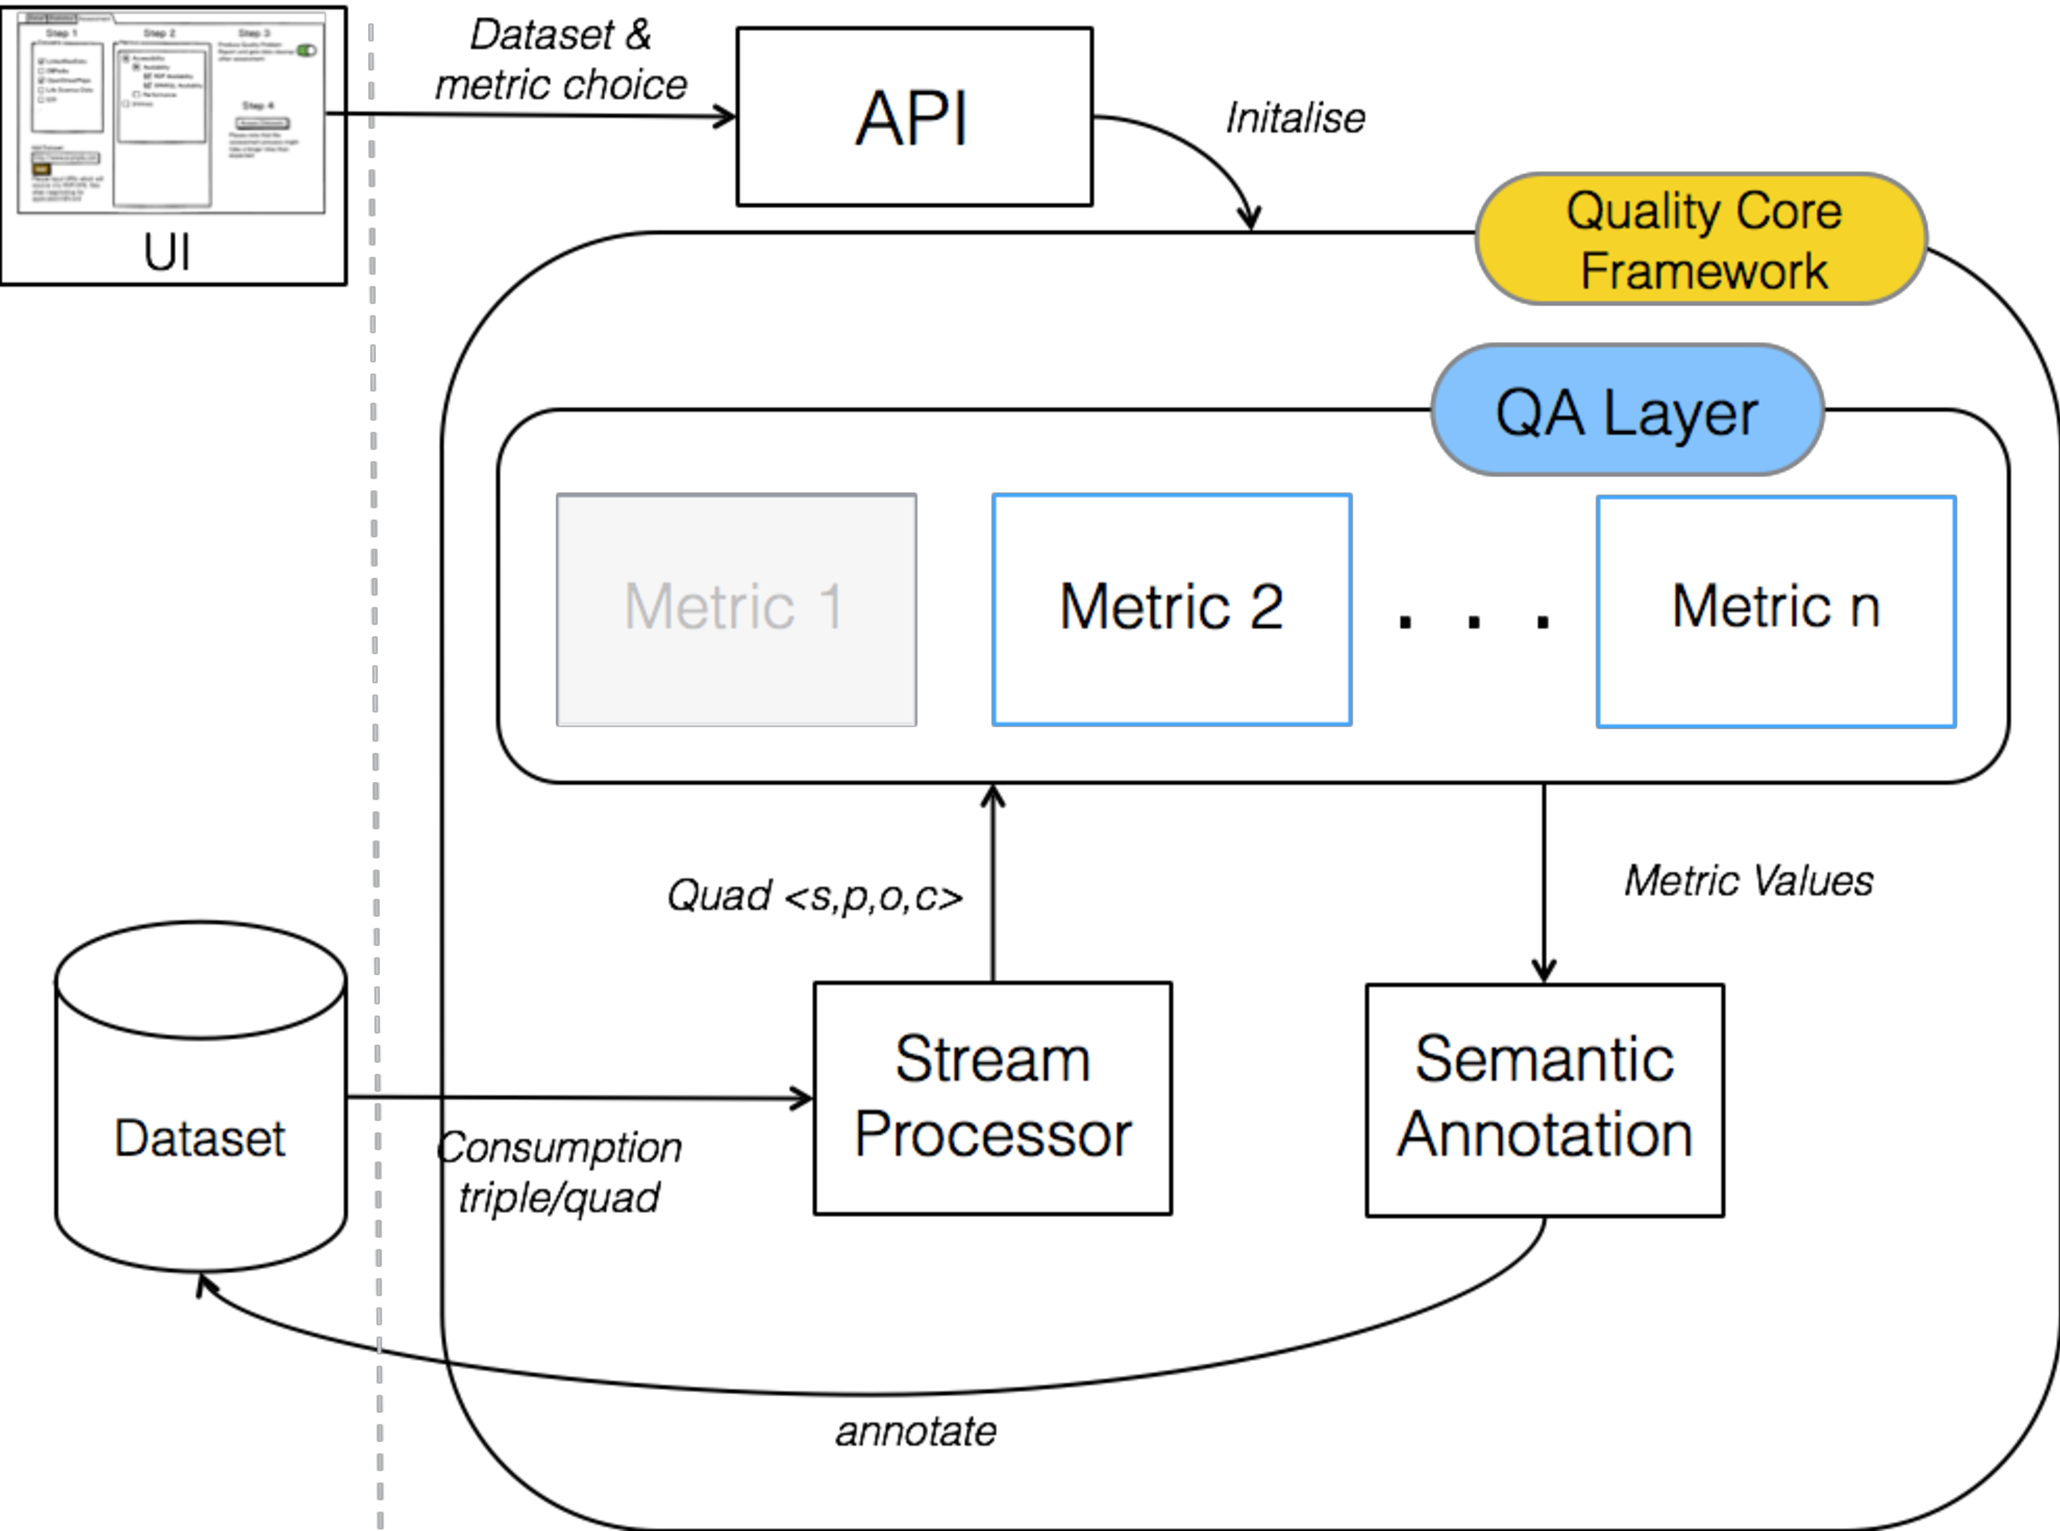
\includegraphics[scale=0.3]{images/closerLook.pdf} 
\caption{Closer look at the Quality Assessment process} 
\label{fig:closerLook}
\end{figure*}

Apache Jena\footnote{\url{http://jena.apache.org}} (cf. Section~\ref{sec:Jena}) provides a dedicated module for reading and writing RDF Data (RDF I/O Technology – RIOT\footnote{\url{http://jena.apache.org/documentation/io/rdf-input.html}}).
The RIOT API functionality provides a number of classes.
Typically the \texttt{RDFDataMgr} is used, which contains the main set of functions to read and load models and datasets.
For the sequential stream processor, the Jena RIOT API was used.

\subsubsection{The Initialisation Process – \texttt{setUpProcess()}}
The first operation on the initialisation is the execution of the \emph{setUpProcess()} method.
Listing~\ref{lst:setUp} is the pseudocode of the the process.
The sequential stream processor starts its initialisation by first trying to identify the serialisation used by the available RDF data dump.
The method \texttt{guessRDFSerialisation} analyses the file serialisation by mapping the file name to one of the RDF serialisations for which Jena has built-in support (e.g. RDF/XML, NTriples, Turtle, NQuads, etc\dots)
According to the file's serialisation, the process then assigns different types of \texttt{PipedRDFIterator}\footnote{\url{https://jena.apache.org/documentation/javadoc/arq/org/apache/jena/riot/lang/PipedRDFIterator.html}} and either a\texttt{PipedQuadsStream}\footnote{\url{https://jena.apache.org/documentation/javadoc/arq/org/apache/jena/riot/lang/PipedQuadsStream.html}} or \texttt{PipedTriplesStream}\footnote{\url{https://jena.apache.org/documentation/javadoc/arq/org/apache/jena/riot/lang/PipedTriplesStream.html}} 
These two objects are required for the scalable execution of the sequential stream processor as together they act as a the ``producer''\footnote{As in the producer in the ``Producer-Consumer problem'' \url{http://en.wikipedia.org/wiki/Producer?consumer_problem}. The consumer is on a separate thread, feeding the metrics.} of sequential RDF triples from the RDF data dump.
Once these are initialised, a flag is set to true to signal that the processor unit is in progress.
Finally, the chosen metrics are loaded into memory.
The loading of metrics is done dynamically during runtime, using the Java specific \texttt{newInstance()}\footnote{\url{http://docs.oracle.com/javase/8/docs/api/java/lang/Class.html#newInstance--}} method. 

\begin{algorithm}
\caption{The Initialisation of the Sequential Stream Process}
\label{lst:setUp}
\begin{algorithmic}[1]
\Procedure{setUpProcess}{}
\State rdfSerialisation = guessRDFSerialisation(datasetURI) ;

\If {rdfSerialisation is Quads} 
\State iterator = new PipedRDFIterator$\langle$Quad$\rangle$() ;
\State rdfStream = new PipedQuadsStream((PipedRDFIterator$\langle$Quad$\rangle$) iterator) ;
\EndIf
\If {rdfSerialisation is Triple} 
\State iterator = new PipedRDFIterator$\langle$Triple$\rangle$() ;
\State rdfStream = new PipedTriplesStream((PipedRDFIterator$\langle$Triple$\rangle$) iterator) ;
\EndIf

\State set initialised boolean to true ;

\State loadMetrics() ;
\EndProcedure
\end{algorithmic}
\end{algorithm}

\subsubsection{The Processing of Triples – \texttt{startProcessing()}}
After the initialisation process, the method \texttt{startProcessing()} is invoked.
The RDFStream \texttt{rdfStream} object starts parsing the RDF dump and producing triple or quad statements in the \texttt{iterator}.
On a different thread, the ``consumer'' – the sequential stream processor – consumes these statements from the \texttt{iterator}, converts them into quads of $\langle s,p,o,c \rangle$, and passes them to all initialised metrics.
The consumption process is repeated until all statements are exhausted from the \texttt{iterator}.
The semantic annotation unit is then signalled to start its annotation.
Listing~\ref{lst:processing} describes this process in pseudocode.

\begin{algorithm}
\caption{Processing Triple/Quad Statements}
\label{lst:processing}
\begin{algorithmic}[1]
\Procedure{startProcessing}{}
\If {initialised == false} \State{throw exception} ; \EndIf

\State create new producer thread for rdfStream ;

\While{(iterator has another statement)} 
\State{quad = Object2Quad(iterator.next()) ;}
\State{pass quad to all metrics and compute metric ;} 
\EndWhile

\State invoke semantic annotation unit ;
\EndProcedure
\end{algorithmic}
\end{algorithm}

\subsubsection{Clean Up – \texttt{cleanUp()}}
The final process is to clean up the objects from memory.
The processor follows a simple approach by assigning \texttt{null} to all objects and shutting down all running threads.

% describe how the stream processor work and the idea behind the processor. 